%!TEX root = ./main.tex
\section{Implementation and Case Studies}
\label{sec5}

\subsection{Implementation}

Our resugaring approach is implemented using PLT Redex\cite{SEwPR}, which is an semantic engineering tool based on reduction semantics\cite{reduction}. The framework of the implementation is as Figure \ref{fig:frame}.
\reduce{figure can be removed}
\begin{figure}[t]
	\centering
	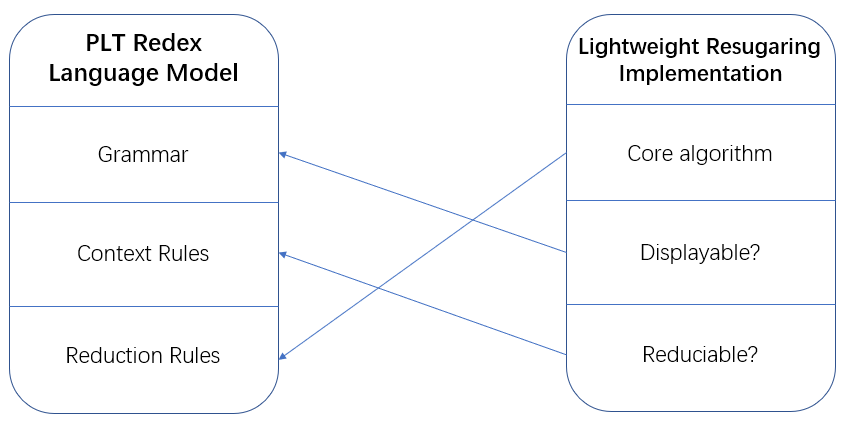
\includegraphics[width=8cm]{images/frame.png}
	\caption{framework of implementation}
	\label{fig:frame}
\end{figure}

In the language model, desugaring rules are written as reduction rules of \m{SurfExp}. And context rules of \m{SurfExp} have no restrict (every subexpressions is reducible as a hole). Then for each resugaring step, we should choose the exact reduction which satisfies the reduction of mixed language's reduction rule  in Section \ref{mark:mixedreduction}.

\label{mark:blackbox}
And one may notice the traditional resugaring approach does not need the whole evaluation rules of core language, a black-box stepper is enough instead. Our approach can also work by  given a black-box stepper with a tricky extension, but a little more information is needed. Here we introduce the extension firstly.
We use $\redc{}{}$ to denote a reduction step of core language's expression in the black-box stepper, and $\rede{}{}$ to denote a step in the extension evaluator for the mixed language. We may use $\redm{}{}$ to denote one-step reduction in our mixed language, defined in the section \ref{mark:mixedreduction}.
\infrule[CoreRed]
{ \forall~i.~e_i\in \m{CoreExp}\\
\redc{(\m{CoreHead}~e_1~\ldots~e_n)}{e'}}
{\rede{(\m{CoreHead}~e_1~\ldots~e_n)}{e'}}
\infrule[CoreExt1]
{ \forall~i.~tmp_i= (e_i \in \m{SurfExp}~?~\m{tmpe}~:~e_i),~where~\m{tmpe}~is~any~reduciable~\m{CoreExp}~term\\
\redc{(\m{CoreHead}~tmp_1~\ldots~tmp_i~\ldots~tmp_n)}{(\m{CoreHead}~tmp_1~\ldots~tmp_i'~\ldots~tmp_n)}}
{\rede{(\m{CoreHead}~e_1~\ldots~e_i~\ldots~e_n)}{(\m{CoreHead}~e_1~\ldots~e_i'~\ldots~e_n)}\\where~\redm{e_i}{e_i'}~if~e_i~\in~\m{SurfExp},~else~\rede{e_i}{e_i'}}
\infrule[CoreExt2]
{ \forall~i.~tmp_i= (e_i \in \m{SurfExp}~?~\m{tmpe}~:~e_i),~where~\m{tmpe}~is~any~reduciable~\m{CoreExp}~term\\
\redc{(\m{CoreHead}~tmp_1~\ldots~tmp_n)}{e'}~\note{// not reduced in subexpressions}}
{\rede{(\m{CoreHead}~e_1~\ldots~e_n)}{e'[e_1/tmp_1~\ldots~e_n/tmp_n]}}
Then we should replace the rules \m{CoreRed1} and \m{CoreRed2} by the following rule.
\infrule[ExtRed]
{\rede{(\m{CoreHead}~e_1~\ldots~e_n)}{e'}}
{\redm{(\m{CoreHead}~e_1~\ldots~e_n)}{e'}}

Putting them in simple words. For expression \Code{(CoreHead $e_1$ $\ldots$ $e_n$)} whose subexpressions contain \m{SurfExp}, replacing all \m{SurfExp} subexpressions not in core language with any reducible core language's term \m{tmpe}. Then getting a result after inputting the new expression $e'$ to the original black-box stepper. If reduction appears at a subexpression at $e_i$ or what the $e_i$ replaced by, then the stepper with the extension should return \Code{(CoreHead $e_1$ $\ldots$ $e_i'$ $\ldots$ $e_n$)}, where $e_i'$ is $e_i$ after the mixed language's one-step reduction ($\redm{}{}$) or after core language's reduction with extension ($\rede{}{}$) (rule \m{CoreExt1}, an example in Figure \ref{fig:e1}). Otherwise, the stepper should return \Code{$e'$}, with all the replaced subexpressions replacing back (rule \m{CoreExt2}, an example in Figure \ref{fig:e2}). The extension will not violate properties of original core language's evaluator. It is obvious that the evaluator with the extension will reduce at the subexpression as it needs in core language, if the reduction appears in a subexpression. One may notice that the stepper with extension behaves the same as mixing the evaluation rules of core language and desugaring rules of surface language. The extension is just to make it works when the evaluator of core language is a black-box stepper, by getting context rules using the \m{tmpe}. That's why the extension is tricky.
\reduce{can be simplified}

\begin{center}
\begin{figure}[thb]
\centering
\Code{(if (and e1 e2) true false)}\\ $\Downarrow_{replace}$\\ \Code{(if tmpe1 true false)}\\ $\Downarrow_{blackbox}$\\ \Code{(if tmpe1' true false)}\\ $\Downarrow_{desugar}$\\ \Code{(if (if e1 e2 false) true false)}
\caption{\m{CoreExt1}'s example}
\label{fig:e1}
\end{figure}

\begin{figure}[thb]
\centering
\Code{(if (if true ture false) (and ...) (or ...))}\\ $\Downarrow_{replace}$ \\\Code{ (if (if true ture false) tmpe2 tmpe3)}\\ $\Downarrow_{blackbox}$\\  \Code{(if true tmpe2 tmpe3)}\\ $\Downarrow_{replaceback}$\\ \Code{(if true (and ...) (or ...))}
\caption{\m{CoreExt2}'s example}
\label{fig:e2}
\end{figure}


\end{center}

But something goes wrong when substitution take place during \m{CoreExt2}. Just as the example we will talk about later in Section \ref{mark:hygienic}, for a expression like \Code{(let (x 2) (Sugar x 1))}, it should reduce to \Code{(Sugar 2 1)} by the \m{CoreRed2} rule, but got \Code{(Sugar x 1)} by the \m{CoreExt2} rule. So when using the extension of black-box stepper's rule (\m{ExtRed2}), we need some other information about in which subexpression a substitution will take place (the substitution can be got by a similar idea as the tricky extension). Then for these subexpressions, we need to do the same substitution before replacing back. 


\label{mark:optimize}
Note that in \m{SurfRed1} rule and \m{CoreExt1} rule, there is a recursive call on $\redm{}{}$. We can optimize the resugaring algorithm by recursively resugaring. For example, \Code{(Sugar1 (Sugar2  ...) ...)} as the input, and find the first subexpression should be reduced. We can firstly get the resugaring sequences of \Code{(Sugar2 ...)}
\begin{Codes}
    (Sugar2 ...)
\OneStep{ exp1}
\DeStep{  expi} \note{// may be 0 or more steps}
\OneStep{ expn}
\end{Codes}
Then a resugaring subsequence is got as
\begin{Codes}
    (Sugar1 (Sugar2 ...) ...)
\OneStep{ (Sugar1 exp1 ...)}
\DeStep{  (Sugar1 expi ...)} \note{// may be 0 or more steps}
\OneStep{ (Sugar1 expn ...)}
\end{Codes}
Thus, we will not need to try to expand the outermost sugar for each inner step (recursively resugaring for inner expression).

As for the automatic derivation of evaluation rules, we implement a simple demo by writing some core language's IFAs (such as \m{if}, \m{let}) manually, because it is enough to do some case studies for the resugaring tasks.
\subsection{Case Studies}

We test some applications on the tool as case studies. Note that we set call-by-value lambda calculus as terms in \m{CommonExp}, because we need to output some intermediate sequences including lambda expressions in some examples. It's easy if we want to skip them.

\subsubsection{simple sugar}
\label{mark:simple}

We construct some simple syntactic sugars and try it on our tool. Some sugar is inspired by the first work of resugaring\cite{resugaring}. The result shows that our approach can handle all sugar features of their first work.
Take a SKI combinator syntactic sugar as an example. We will show why our approach is efficient.
\[
\begin{array}{l}
\drule{\m{S}}{\Code{(lambdaN (x1 x2 x3) (x1 x2 (x1 x3)))}}\\
\drule{\m{K}}{\Code{(lambdaN (x1 x2) x1)}}\\
\drule{\m{I}}{\Code{(lambdaN (x) x)}}
\end{array}
\]




Although SKI combinator calculus is a reduced version of lambda calculus, we can construct combinators' sugar based on call-by-need lambda calculus in our core language. For sugar expression \Code{(S (K (S I)) K xx yy)}, we get the following resugaring sequences.
\begin{Codes}
    (S (K (S I)) K xx yy)
\OneStep (((K (S I)) xx (K xx)) yy)
\OneStep (((S I) (K xx)) yy)
\OneStep (I yy ((K xx) yy))
\OneStep (yy ((K xx) yy))
\OneStep (yy xx)
\end{Codes}


For the traditional approach, the sugar expression should firstly desugar to
\begin{Codes}
((lambdaN (x1 x2 x3) (x1 x3 (x2 x3)))
  ((lambdaN (x1 x2) x1)
   ((lambdaN  (x1 x2 x3) (x1 x3 (x2 x3)))
    (lambdaN (x) x)))
  (lambdaN (x1 x2) x1)
  xx yy)
\end{Codes}
\reduce{can be removed}

Then in our core language, the execution of expanded expression will contain 33 reduction steps in our implementation. For each step, there will be many attempts to match and substitute the syntactic sugars to resugar the expression. It will omit more steps for a larger expression.

As for the derivation of syntactic sugar's evaluation rules, we have shown an example of \m{and} sugar and \m{or} sugar in overview. But what if the \m{or} sugar written as follows?
\[\drule{\Code{(Or $e_1$ $e_2$)}}{\Code{(let (x $e_1$) (if x x $e_2$))}}\]
Of course, we got the same evaluation rules as the example in overview.
\[
\begin{array}{c}
\infer {(\mbox{or}~e_1~e_2) \rightarrow (\mbox{or}~e_1'~e_2)} {e_1~ \rightarrow~e_1'}
\qquad
(\mbox{or}~\#t~e2) \rightarrow \#t
\quad
(\mbox{or}~\#f~e2) \rightarrow e_2 \\
\end{array}
\]

Then for expressions headed with \m{or}, we won't need the one-step try to figure out whether desugaring or processing on a subexpression, which makes our approach more concise. Overall, the unidirectional resugaring algorithm makes our approach efficient, because no attempts for resugaring the expression are needed.
\subsubsection{hygienic sugar}
\label{mark:hygienic}


The second work\cite{hygienic} of traditional resugaring approach mainly processes hygienic sugar compared to first work. It uses a DAG to represent the expression. However, hygiene is not hard to be handled by our lazy desugaring strategy. Our algorithm can easily process hygienic sugar without special data structure.
A typical hygienic problem is as the following example.
\[
\drule{\Code{(Hygienicadd $e_1$ $e_2$)}}{\Code{(let (x $e_1$) (+ x $e_2$))}}
\]
% \begin{Codes}
% 	(Hygienicadd e1 e2) \DeStep{ (let ((x e1)) (+ x e2))}
% \end{Codes}
For traditional resugaring approach, if we want to get sequences of \Code{(let (x 2) (Hygienicadd 1 x))}, it will firstly desugar to \Code{(let (x 2) (let (x 1) (+ x x)))}, which is awful because the two $x$ in \Code{(+ x x)} should be bind to different value. So the traditional hygienic resugaring approach use abstract syntax DAG to distinct different \m{x} in the desugared expression. But for our approach based on lazy desugaring, the \m{hygienicadd} sugar does not have to desugar until necessary, thus, getting following sequences based on a  rewriting system which renaming the variables during the rewriting.

\begin{Codes}
    (let (x 2) (Hygienicadd 1 x))
\OneStep{ (Hygienicadd 1 2)}
\OneStep{ (+ 1 2)}
\OneStep{ 3}
\end{Codes}

The lazy desugaring is also convenient for hygienic resugaring for non-hygienic rewriting. For example, \Code{(let (x 1) (+ x (let (x 2) (+ x 1))))} may be reduced to \Code{(+ 1 (let (1 2) (+ 1 1)))} by a simple core language whose \Code{let} expression does not handle cases like that. But by writing a simple sugar Let,
\[\drule{\Code{(Let~$e_1$~$e_2$~$e_3$)}}{\Code{(let~($e_1$~$e_2$)~$e_3$)}}\]
and making some simple modifies in the reduction of mixed language, we will get the following sequences in our system.
\begin{Codes}
    (Let x 1 (+ x (Let x 2 (+ x 1))))
\OneStep{ (Let x 1 (+ x (+ 2 1)))}
\OneStep{ (Let x 1 (+ x 3))}
\OneStep{ (+ 1 3)}
\OneStep{ 4}
\end{Codes}

In practical application, we think hygiene can be easily processed by rewriting systems, so we just use a rewriting system which can rename variable automatically. 

And for the derivation method, there is no rewriting system at all, but the hygiene is handled more concisely. we build a hygienic sugar \m{Hygienicor} based the \m{or} sugar.
\[
\begin{array}{l}
\drule{\Code{(Or $e_1$ $e_2$)}}{\Code{(let (x $e_1$) (if x x $e_2$))}}\\
\drule{\Code{(Hygienicor $e_1$ $e_2$)}}{\Code{(let (x $e_1$) (or $e_2$ x))}}
\end{array}
\]
Though no need to write the sugar like that, something wrong may happen without hygienic rewriting system (\Code{(if x x x)} appears). But by the method introduced in \todo{..}, we can easily get the following rules, which will behave as it should be in resugaring.
\[
\begin{array}{c}
\infer {(\mbox{Hygienicor}~e_1~e_2) \rightarrow (\mbox{Hygienicor}~e_1'~e_2)} {e_1~ \rightarrow~e_1'}
\qquad
\infer {(\mbox{Hygienicor}~v_1~e_2) \rightarrow (\mbox{Hygienicor}~v_1~e_2')} {e_2~ \rightarrow~e_2'}
\\
(\mbox{Hygienicor}~v_1~\#t) \rightarrow \#t
\quad
(\mbox{Hygienicor}~v_1~\#f) \rightarrow v_1\\
\end{array}
\]

Overall, our result shows lazy desugaring is really a good way to handle hygienic sugar in any systems.

\subsubsection{recursive sugar}
\label{sec:recursiveSugar}

Recursive sugar is a kind of syntactic sugars where call itself or each other during the expanding. For example,
\[
\begin{array}{l}
\drule{(\m{Odd}~$e$)~}{\Code{(if (> $e$ 0) (Even (- $e$ 1)) \false)}}\\
\drule{(\m{Even}~$e$)}{\Code{(if (> $e$ 0) (Odd (- $e$ 1)) \true)}}
\end{array}
\]
are common recursive sugars. The traditional resugaring approach can't process syntactic sugar written as this (non pattern-based) easily, because boundary conditions are in the sugar itself.

Take \Code{(Odd 2)} as an example. The previous work will firstly desugar the expression using the rewriting system. Then the rewriting system will never terminate as following shows.
\begin{Codes}
   (Odd 2)
\DeStep{ (if (> 2 0) (Even (- 2 1) \#f))}
\DeStep{ (if (> (- 2 1) 0) (Odd (- (- 2 1) 1) \#t))}
\DeStep{ (if (> (- (- 2 1) 1) 0) (Even (- (- (- 2 1) 1) 1) \#f))}
\DeStep{ ...}
\end{Codes}


Then the advantage of our approach is embodied. Our lightweight approach doesn't require a whole expanding of sugar expression, which gives the framework chances to judge boundary conditions in sugars themselves, and showing more intermediate sequences. We get the resugaring sequences of the former example using our tool.
\begin{Codes}
    (Odd 2)
\OneStep{ (Even (- 2 1))}
\OneStep{ (Even 1)}
\OneStep{ (Odd (- 1 1))}
\OneStep{ (Odd 0)}
\OneStep{ \#f}
\end{Codes}


We also construct some higher-order syntactic sugars and test them. The higher-order feature is important for constructing practical syntactic sugars. And many higher-order sugars should be constructed by recursive definition. The first sugar is \m{filter}, implemented by pattern matching term rewriting.
\[\begin{array}{l}
\drule{\Code{(filter $e$ (list $v_1$ $v_2$ ...))}}{}\\
\qquad\Code{(if ($e$ $v_1$) (cons $v_1$ (filter $e$ (list $v_2$ ...)))\ (filter $e$ (list $v_2$ ...)))}\\
\drule{\Code{(filter $e$ (list))}}{\Code{(list)}}
\end{array}\]

and getting the following result.

\begin{Codes}
    (filter (lambda (x) (and (> x 1) (< x 4))) (list 1 2 3 4))
\OneStep{ (filter (lambda (x) (and (> x 1) (< x 4))) (list 2 3 4))}
\OneStep{ (cons 2 (filter (lambda (x) (and (> x 1) (< x 4))) (list 3 4)))}
\OneStep{ (cons 2 (cons 3 (filter (lambda (x) (and (> x 1) (< x 4))) (list 4))))}
\OneStep{ (cons 2 (cons 3 (filter (lambda (x) (and (> x 1) (< x 4))) (list))))}
\OneStep{ (cons 2 (cons 3 (list)))}
\OneStep{ (cons 2 (list 3))}
\OneStep{ (list 2 3)}
\end{Codes}
Here, although the sugar can be processed by traditional resugaring approach, it will be redundant. The reason is that, a filter for a list of length $n$ will match to find possible resugaring $n*(n-1)/2$ times. Thus, lazy desugaring is really important to reduce the resugaring complexity of recursive sugar.

Moreover, just like the \emph{Odd and Even} sugar above, there are some simple rewriting systems which do not allow pattern-based rewriting. Or there are some sugars which need to be expressed by the terms in core language as rewriting conditions. Take the example of another higher-order sugar \m{map} as an example.
\[
\begin{array}{l}
\drule{\Code{(map $e_1$ $e_2$)}}{}\\
\Code{(let (x $e_2$) (if (empty? x) (list) (cons ($e_1$ (first x)) (map $e_1$ (rest x)))))}
\end{array}
\]
and get following resugaring sequences.
\begin{Codes}
    (map (lambda (x) (+ x 1)) (cons 1 (list 2)))
\OneStep{ (map (lambda (x) (+ x 1)) (list 1 2))}
\OneStep{ (cons 2 (map (lambda (x) (+ 1 x)) (list 2)))}
\OneStep{ (cons 2 (cons 3 (map (lambda (x) (+ 1 x)) (list))))}
\OneStep{ (cons 2 (cons 3 (list)))}
\OneStep{ (cons 2 (list 3))}
\OneStep{ (list 2 3)}
\end{Codes}

Note that the \m{let} term is to limit the subexpression only appears once in RHS. In this example, we can find that the list \Code{(cons 1 (list 2))}, though equal to \Code{(list 1 2)}, is represented by core language's term. So it will be difficult to handle such inline boundary conditions by rewriting system. But our approach is easy to handle cases like this. So our resugaring approach by lazy desugaring is powerful.
